\documentclass[a4paper]{article}

\usepackage{fullpage} % Package to use full page
\usepackage{parskip} % Package to tweak paragraph skipping
\usepackage{amsmath}
\usepackage{amssymb}
\usepackage{hyperref}
\usepackage{subcaption}
\usepackage{graphicx}

\title{16-720B Computer Vision: Homework 3 \\
Lucas-Kanade Tracking and Correlation Filters}
\author{Heethesh Vhavle\\
Andrew ID: hvhavlen}
\date{24 October 2018}

\begin{document}

\maketitle

\section{Lucas-Kanade Tracking}
\subsubsection*{1.1.1}
$\frac { \partial \mathcal { W } ( \mathbf { x } ; \mathbf { p } ) } { \partial \mathbf { p } ^ { T } }$ represents the Jacobian of the warped image. For a pure translation the Jacobian is as follows.
\begin{gather}
    \frac { \partial \mathcal { W } ( \mathbf { x } ; \mathbf { p } ) } { \partial \mathbf { p } ^ { T } } = \left( \begin{array} { l l l l } { 1 } & { 0 } \\ { 0 } & { 1 } \end{array} \right)
\end{gather}

\subsubsection*{1.1.2}
We can linearize the objective function locally by first-order Taylor expansion and can rewrite and rearrange our equation to minimize as follows.
\begin{gather}
\begin{array}{c}
\arg \min _ { \Delta \mathbf { p } } \sum _ { \mathbf { x } \in \mathbb { N } } \left\| \mathcal { I } _ { t + 1 } ( \mathbf { x } ^ { \prime } + \Delta \mathbf { p } ) - \mathcal { I } _ { t } ( \mathbf { x } ) \right\| _ { 2 } ^ { 2 }
& \\
where \;\; \mathcal { I } _ { t + 1 } \left( \mathbf { x } ^ { \prime } + \Delta \mathbf { p } \right) \approx \mathcal { I } _ { t + 1 } \left( \mathbf { x } ^ { \prime } \right) + \frac { \partial \mathcal { I } _ { t + 1 } \left( \mathbf { x } ^ { \prime } \right) } { \partial \mathbf { x } ^ { \prime T } } \frac { \partial \mathcal { W } ( \mathbf { x } ; \mathbf { p } ) } { \partial \mathbf { p } ^ { T } } \Delta \mathbf { p }
& \\
\arg \min _ { \Delta \mathbf { p } } \sum _ { \mathbf { x } \in \mathbb { N } } \left\| \mathcal { I } _ { t + 1 } \left( \mathbf { x } ^ { \prime } \right) + \frac { \partial \mathcal { I } _ { t + 1 } \left( \mathbf { x } ^ { \prime } \right) } { \partial \mathbf { x } ^ { \prime T } } \frac { \partial \mathcal { W } ( \mathbf { x } ; \mathbf { p } ) } { \partial \mathbf { p } ^ { T } } \Delta \mathbf { p } - \mathcal { I } _ { t } ( \mathbf { x } ) \right\| _ { 2 } ^ { 2 }
& \\
\arg \min _ { \Delta \mathbf { p } } \sum _ { \mathbf { x } \in \mathbb { N } } \left\| \frac { \partial \mathcal { I } _ { t + 1 } \left( \mathbf { x } ^ { \prime } \right) } { \partial \mathbf { x } ^ { \prime T } } \frac { \partial \mathcal { W } ( \mathbf { x } ; \mathbf { p } ) } { \partial \mathbf { p } ^ { T } } \Delta \mathbf { p } - \left( \mathcal { I } _ { t } ( \mathbf { x } ) - \mathcal { I } _ { t + 1 } \left( \mathbf { x } ^ { \prime } \right) \right )\right\| _ { 2 } ^ { 2 }
& \\
\arg \min _ { \Delta \mathbf { p } } \| \mathbf { A } \Delta \mathbf { p } - \mathbf { b } \| _ { 2 } ^ { 2 }
\end{array}
\end{gather}

Comparing the last two forms above we get the following.
\begin{gather}
    \begin{array}{c}
    \mathbf { A } = \sum _ { \mathbf { x } \in \mathbb { N } } \frac { \partial \mathcal { I } _ { t + 1 } \left( \mathbf { x } ^ { \prime } \right) } { \partial \mathbf { x } ^ { \prime T } } \frac { \partial \mathcal { W } ( \mathbf { x } ; \mathbf { p } ) } { \partial \mathbf { p } ^ { T } }
    &  \\
    \mathbf { b } = \sum _ { \mathbf { x } \in \mathbb { N } } \mathcal { I } _ { t } ( \mathbf { x } ) - \mathcal { I } _ { t + 1 } \left( \mathbf { x } ^ { \prime } \right)
    \end{array}
\end{gather}

In other words, \textbf{A} represents the steepest descent images and \textbf{b} represents the error image.

\subsubsection*{1.1.3}
To minimize $\Delta \mathbf { p }$ in equation 2, we take its first derivative and equate it to zero.
\begin{gather}
    \begin{array}{c}
    \sum _ { \mathbf { x } \in \mathbb { N } } 2\mathbf { A } ^ {\top} (\mathbf { A } \Delta \mathbf { p } - \mathbf { b }) = 0
    &  \\
    \sum _ { \mathbf { x } \in \mathbb { N } } \mathbf { A } ^ {\top} \mathbf { A } \Delta \mathbf { p } = \sum _ { \mathbf { x } \in \mathbb { N } } \mathbf { A } ^ {\top} \mathbf { b }
    &  \\ 
    \Delta \mathbf { p } = \sum _ { \mathbf { x } \in \mathbb { N } } (\mathbf { A } ^ {\top} \mathbf { A }) ^ {-1} \mathbf { A } ^ {\top} \mathbf { b }
    \end{array}
\end{gather}

As it can be seen above, in order to solve for $\Delta \mathbf { p }$, $\mathbf { A } ^ { T } \mathbf { A }$ must be invertible or non-singular matrix or must have a non-zero determinant to obtain an unique solution for $\Delta \mathbf { p }$.

\subsection*{1.3 \hspace{4.5} Car Sequence Tracking}
\begin{figure}[!ht]
\centering
\begin{tabular}{ccc}
{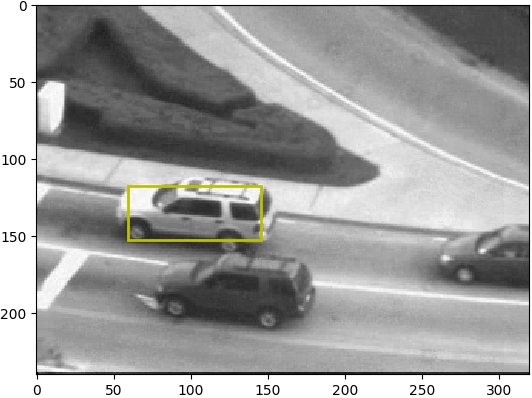
\includegraphics[width=0.3\textwidth]{images/carseq_1}} &
{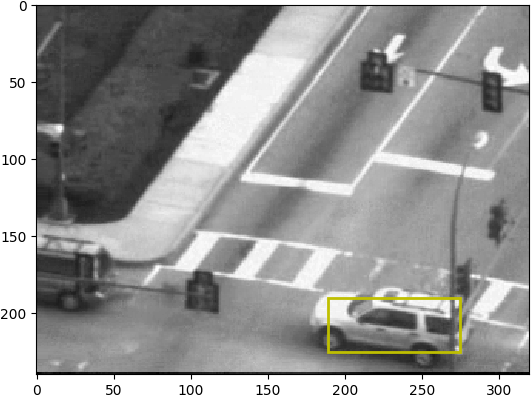
\includegraphics[width=0.3\textwidth]{images/carseq_100}} &
{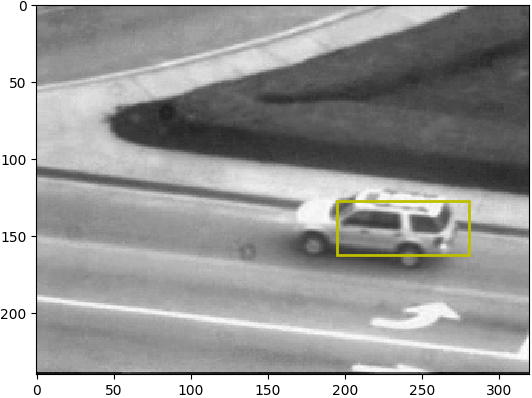
\includegraphics[width=0.3\textwidth]{images/carseq_200}}
\end{tabular}
\begin{tabular}{cc}
{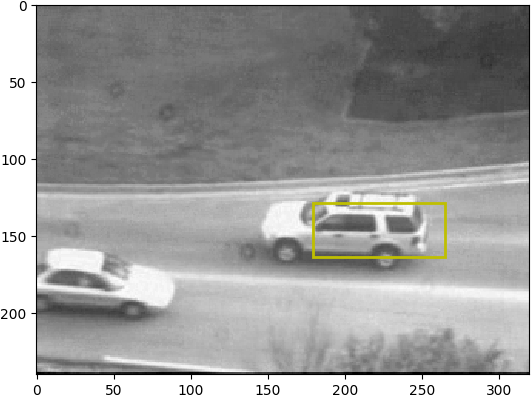
\includegraphics[width=0.3\textwidth]{images/carseq_300}} &
{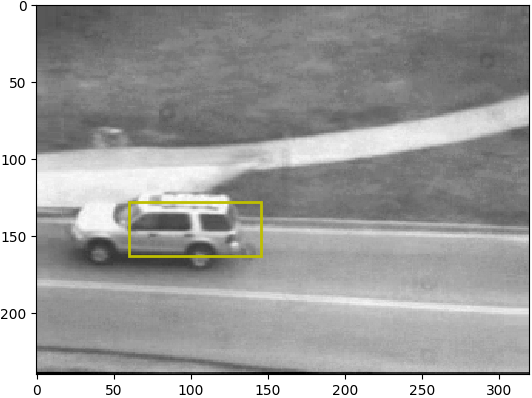
\includegraphics[width=0.3\textwidth]{images/carseq_400}}
\end{tabular}
\caption{Lucas-Kanade Tracking with One Single Template at Frames 1, 100, 200, 300, 400}
\end{figure}

\subsection*{1.4 \hspace{4.5} Car Sequence Tracking with Template Drift Correction}
We are using Strategy 3 for template drift correction here. Since the template is updated every frame and registered to the initial template (drift correction), the object is tracked correctly till the end and improves the tracking robustness compared to the original Lucas-Kanade. If we implement this using Lucas-Kanade with Affine Transform, we can achieve even better resuts compared to the current pure translation case.

\newpage
\begin{figure}[!ht]
\centering
\begin{tabular}{ccc}
{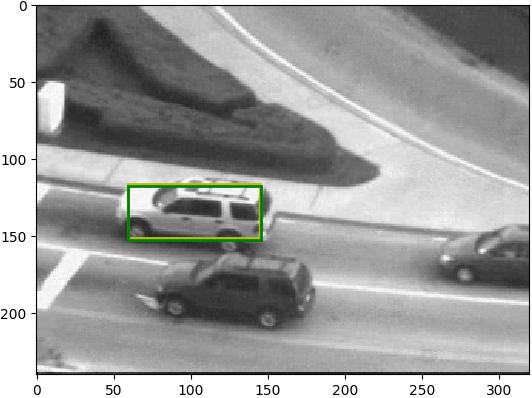
\includegraphics[width=0.3\textwidth]{images/carseqrects-wcrt_1}} &
{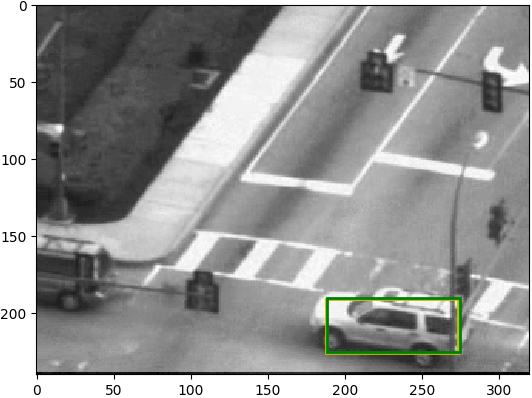
\includegraphics[width=0.3\textwidth]{images/carseqrects-wcrt_100}} &
{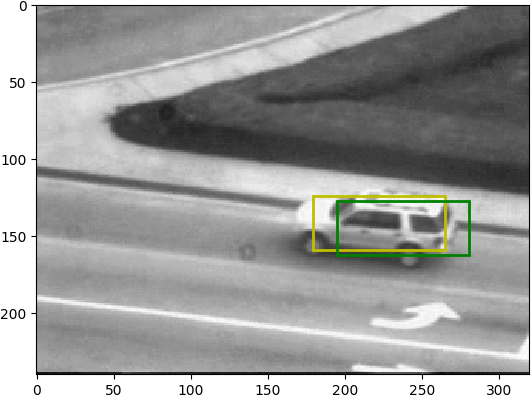
\includegraphics[width=0.3\textwidth]{images/carseqrects-wcrt_200}}
\end{tabular}
\begin{tabular}{cc}
{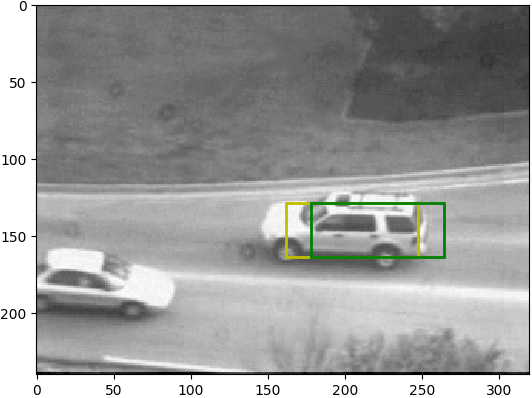
\includegraphics[width=0.3\textwidth]{images/carseqrects-wcrt_300}} &
{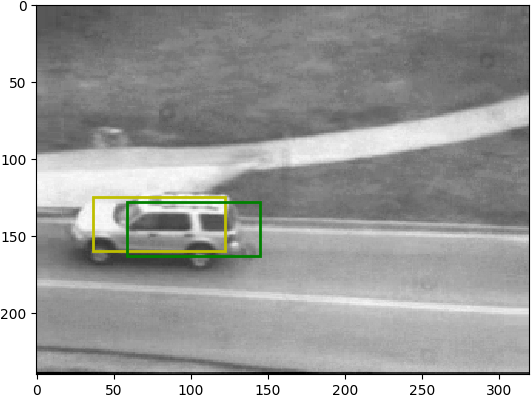
\includegraphics[width=0.3\textwidth]{images/carseqrects-wcrt_400}}
\end{tabular}
\caption{Lucas-Kanade Tracking with Template Drift Correction at Frames 1, 100, 200, 300, 400}
\end{figure}

\section{Lucas-Kanade Tracking with Appearance Basis}
\subsection{Appearance Basis}
Given a set of \textit{k} image basis $\left\{ \mathcal { B } _ { k } \right\} _ { k = 1 } ^ { K }$ weighted by $\mathbf { w } = \left[ w _ { 1 } , \dots , w _ { K } \right] ^ { T }$, we have the following relation.
\begin{gather}
\mathcal { I } _ { t + 1 } ( \mathbf { x } ) = \mathcal { I } _ { t } ( \mathbf { x } ) + \sum _ { k = 1 } ^ { K } w _ { k } \mathcal { B } _ { k } ( \mathbf { x } )
\end{gather}

Reorganizing this and expanding the summation.
\begin{gather}
\begin{array}{c}
\mathcal { I } _ { t + 1 } ( \mathbf { x } ) - \mathcal { I } _ { t } ( \mathbf { x } ) = w _ { 1 } \mathcal { B } _ { 1 } ( \mathbf { x } ) + \dots + w _ { k } \mathcal { B } _ { k } ( \mathbf { x } ) + \dots + w _ { K } \mathcal { B } _ { K } ( \mathbf { x } )
&  \\
\end{array}    
\end{gather}

Multiplying both sides by $\mathcal { B } _ { k } ( \mathbf { x } )$ and using the orthogonal property of basis we get the following.
\begin{gather}
    \mathcal { B } _ { k } ( \mathbf { x } )(\mathcal { I } _ { t + 1 } ( \mathbf { x } ) - \mathcal { I } _ { t } ( \mathbf { x } )) = 0 + \dots + w _ { k } \mathcal { B } _ { k } ( \mathbf { x } ) \mathcal { B } _ { k } ( \mathbf { x } ) + \dots + 0
\end{gather}

Reorganizing the above equation we can express any $\left\{ w _ { k } \right\} _ { k = 1 } ^ { K }$ as follows.
\begin{gather}
w _ { k } = \frac{\mathcal { B } _ { k } ( \mathbf { x } ) (\mathcal { I } _ { t + 1 } ( \mathbf { x } ) - \mathcal { I } _ { t } ( \mathbf { x } ))}{\| \mathcal { B } _ { k } ( \mathbf { x } ) \| ^ { 2 }}
\end{gather}
\begin{gather}
    w _ { k } = \mathcal { B } _ { k } ( \mathbf { x } ) (\mathcal { I } _ { t + 1 } ( \mathbf { x } ) - \mathcal { I } _ { t } ( \mathbf { x } ))
\end{gather}

\newpage
\subsection*{2.3 \hspace{4.5} Tracking Results}
In this case, the results Lucas-Kanade Tracking and Lucas-Kanade Tracking with Appearance Basis seems to be very similar. But if we consider another scenario with greater variation in appearance or illumination of the object to be tracked, the Appearance Basis method will definitely give better results.
\begin{figure}[!ht]
\centering
\begin{tabular}{ccc}
{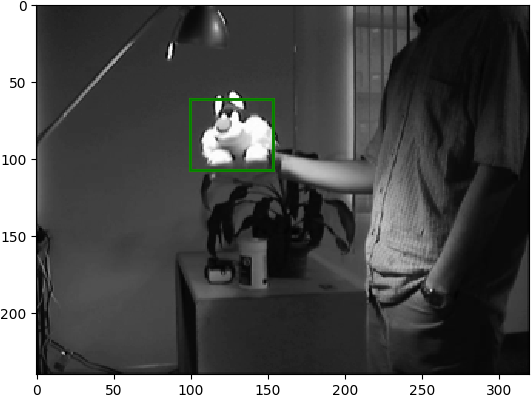
\includegraphics[width=0.3\textwidth]{images/sylvseqrects_1}} &
{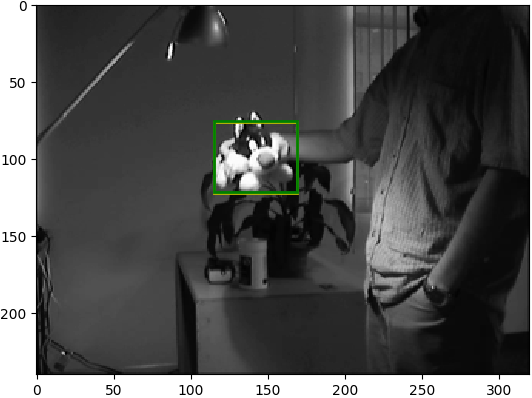
\includegraphics[width=0.3\textwidth]{images/sylvseqrects_200}} &
{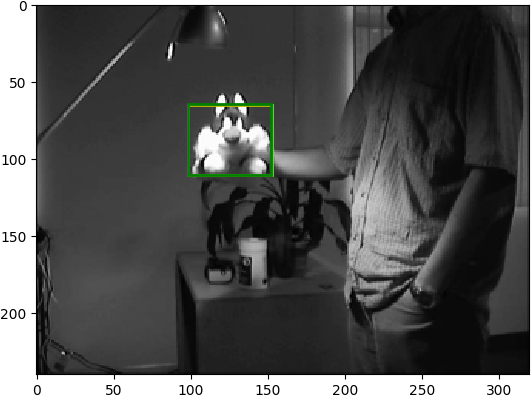
\includegraphics[width=0.3\textwidth]{images/sylvseqrects_300}}
\end{tabular}
\begin{tabular}{cc}
{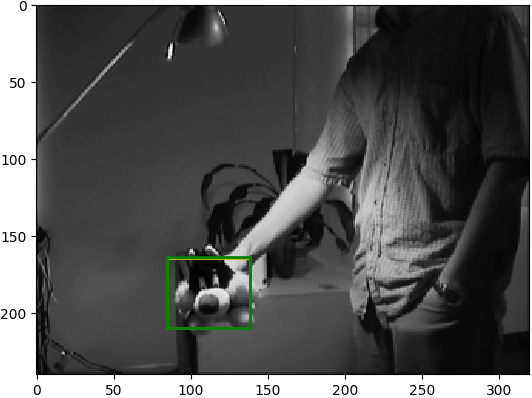
\includegraphics[width=0.3\textwidth]{images/sylvseqrects_350}} &
{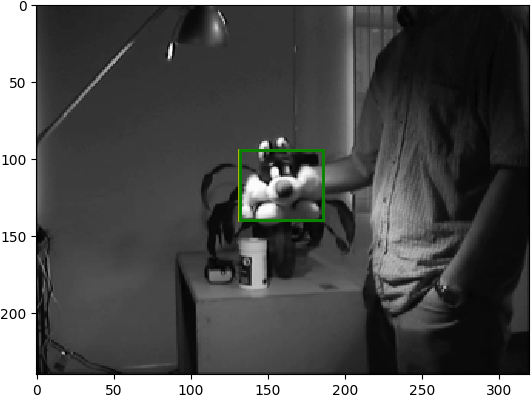
\includegraphics[width=0.3\textwidth]{images/sylvseqrects_400}}
\end{tabular}
\caption{Lucas-Kanade Tracking with Appearance Basis at Frames 1, 200, 300, 350, 400}
\end{figure}

\section{Affine Motion Subtraction}
\begin{figure}[!ht]
\centering
\begin{tabular}{cc}
{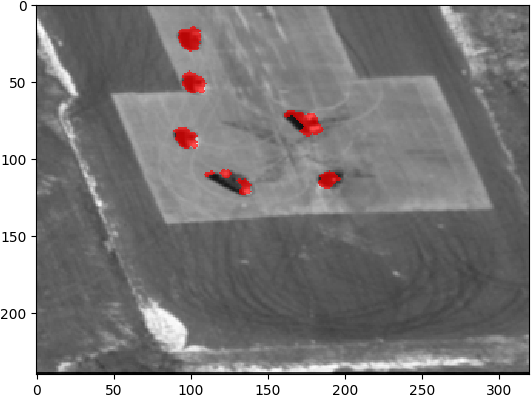
\includegraphics[width=0.35\textwidth]{images/aerialseq_30}} &
{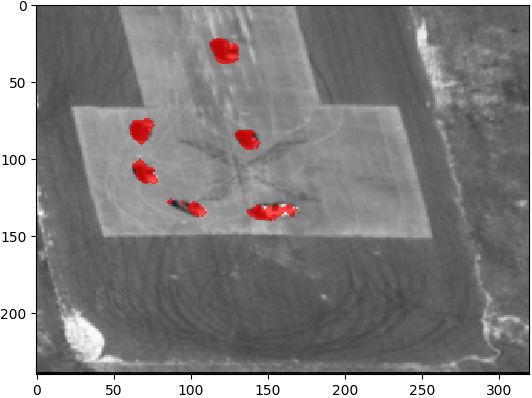
\includegraphics[width=0.35\textwidth]{images/aerialseq_60}}
\end{tabular}
\begin{tabular}{cc}
{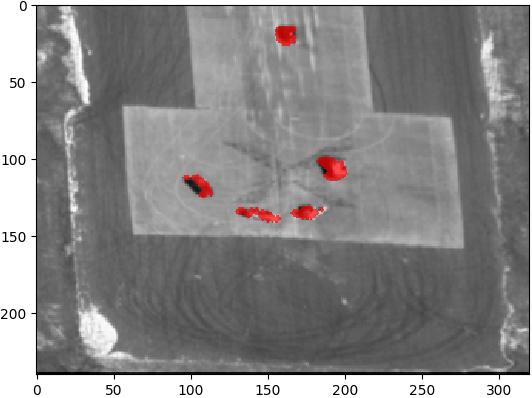
\includegraphics[width=0.35\textwidth]{images/aerialseq_90}} &
{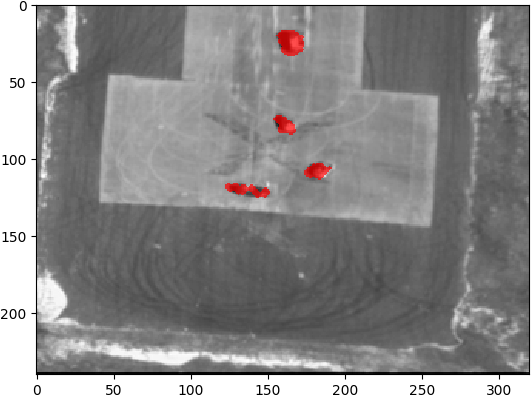
\includegraphics[width=0.35\textwidth]{images/aerialseq_120}}
\end{tabular}
\caption{Result of Dominant Motion Subtraction after Lucas-Kanade Registration with Affine Transform at Frames 30, 60, 90, 120}
\end{figure}

\section{Efficient Tracking}
\subsection{Inverse Composition}

In Lucas-Kanade Inverse Composition, we are swapping the template and the current image and the image registration is done the other way around. Thus, there are certain steps of original Lucas-Kanade (steps 3-6) that can be computed only once without re-computing them in every iteration. The steps that we move out of the iteration also involves computationally costly Hessian calculation, which we are keeping as a constant and computing only once now. This along with its operations such as calculating gradients, multiplying with the Jacobian to get the steepest descent images and so on are consequently moved out of the loop. Thus, the Inverse Composition method is more efficient than the original method.

\subsection{Correlation Filters}
We need to minimize the following equation where $\mathbf { X } = \left[ \mathbf { x } _ { 1 } , \ldots , \mathbf { x } _ { N } \right]$ is a set of sub-images from Lena image and $\mathbf { x } _ { n } \in \mathbb { R } ^ { D }$ (\textit{D} = 1305). $\mathbf { y } = \left[ y _ { 1 } , \ldots , y _ { N } \right]$ are the output labels, where $y _ { n }$ lies between zero and one. We need to find the resultant linear discriminant weight vector \textbf{g} for the penalty values $\lambda = 0$ and $\lambda = 1$. We can expand the terms of the equation as follows.
\begin{gather}
\frac{1}{2} \| \mathbf { y } - \boldsymbol { X } ^ { \top } \mathbf { g } \| _ { 2 } ^ { 2 } + \frac{1}{2} \lambda \| \mathbf { g } \| _ { 2 } ^ { 2 }
\\
\begin{array}{c}
&= ( \mathbf { y } - \boldsymbol { X } ^ { \top } \mathbf { g } ) ^ { \top } ( \mathbf { y } - \boldsymbol { X } ^ { \top } \mathbf { g } ) + \lambda \mathbf { g } ^ { \top } \mathbf { g } 
\\
&= \mathbf { y } ^ { \top } \mathbf { y } - \left( \boldsymbol { X } \mathbf { y } \right) ^ { \top } \mathbf { g } - \mathbf { g } ^ { \top } \boldsymbol { X } \mathbf { y } + \mathbf { g } ^ { \top } \boldsymbol { X } \boldsymbol { X } ^ { \top } \mathbf { g } + \lambda \mathbf { g } ^ { \top } \mathbf { g }
\end{array}
\end{gather}

The following identities of Matrix Calculus can be used. \textbf{A} and \textbf{b} are not functions of \textbf{x}.
\begin{gather}
\begin{array}{c}
    & \frac { \partial \mathbf { b } ^ { \top } \mathbf { A } \mathbf { x } } { \partial \mathbf { x } } = \mathbf { A } ^ { \top } \mathbf { b }
    &  \\
    \frac { \partial \mathbf { x } ^ { \top } \mathbf { A } \mathbf { x } } { \partial \mathbf { x } } = \left( \mathbf { A } + \mathbf { A } ^ { \top } \right) \mathbf { x }
    & \\
    \frac { \partial \mathbf { x } ^ { \top } \mathbf { a } } { \partial \mathbf { x } } = \mathbf { a }
    & \\
    \frac { \partial \mathbf { x } ^ { \top } \mathbf { x } } { \partial \mathbf { x } } = \mathbf { 2x }
\end{array}
\end{gather}

In order to do find the value of \textbf{g} to minimize the equation 10, we can find its derivative and equate it to zero. Also setting $\mathbf{S} = \mathbf{X}\mathbf{X} ^ {\top}$ and simplifying the terms. $\mathbf{S}$ here is a symmetric matrix.
\begin{gather}
    \begin{array} { c } { \frac { \partial } { \partial \mathbf { g } } \left( \mathbf { y } ^ { \top } \mathbf { y } - \left( \boldsymbol { X } \mathbf { y } \right) ^ { \top } \mathbf { g } - \mathbf { g } ^ { \top } \boldsymbol { X } \mathbf { y } + \mathbf { g } ^ { \top } \boldsymbol { S } \mathbf { g } + \lambda \mathbf { g } ^ { \top } \mathbf { g } \right) } 
    \\ 
    { &= - 2 \left( \boldsymbol { X } \mathbf { y } \right) + \left( \boldsymbol { S } + \left( \boldsymbol { S } \right) ^ { \top } \right) \mathbf { g } + 2 \lambda \mathbf { g } }
    \\ 
    { &= - 2 \boldsymbol { X } \mathbf { y } + 2 \boldsymbol { S } \mathbf { g } + 2 \lambda \mathbf { g } } \end{array}
\end{gather}

\begin{gather}
    \begin{aligned} - 2 \boldsymbol { X } \mathbf { y } + 2 \boldsymbol { S } \mathbf { g } + 2 \lambda \mathbf { g } & = 0
    \\ 
    \boldsymbol { S } \mathbf { g } + \lambda \mathbf { g } & = \boldsymbol { X } \mathbf { y }
    \\ 
    \left( \boldsymbol { S } + \lambda \boldsymbol { I } \right) \mathbf { g } & = \boldsymbol { X } \mathbf { y }
    \end{aligned}
\end{gather}

If $\left( \boldsymbol { S } + \lambda \boldsymbol { I } \right)$ is invertible with non-zero determinant, we can obtain the required form of equation as follows.
\begin{gather}
    \mathbf { g } = \left( \boldsymbol { S } + \lambda \boldsymbol { I } \right) ^ { - 1 } \boldsymbol { X } \mathbf { y }
\end{gather}

\subsection{Filter Responses using Correlation}
\begin{figure}[!ht]
\centering
\begin{tabular}{cc}
{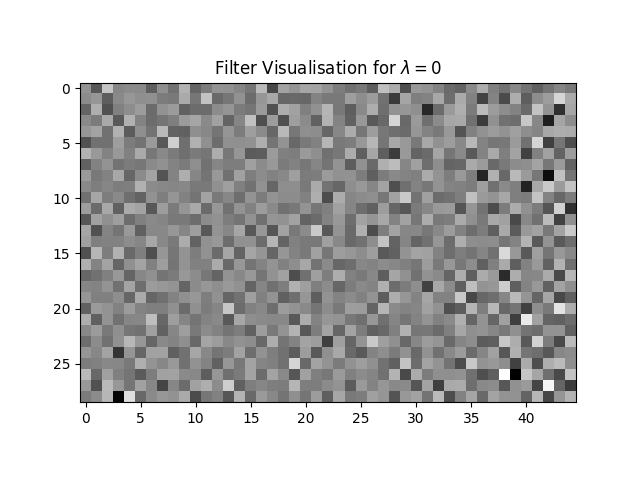
\includegraphics[width=0.45\textwidth]{corr-filters/g0_fliter}} &
{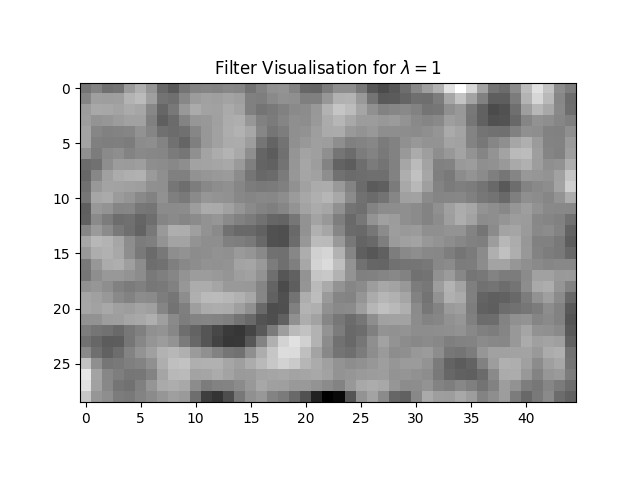
\includegraphics[width=0.45\textwidth]{corr-filters/g1_fliter}}
\end{tabular}
\caption{Resultant Linear Discriminant Weight Vector for $\lambda = 0, 1$}
\end{figure}

\begin{figure}[!ht]
\centering
\begin{tabular}{cc}
{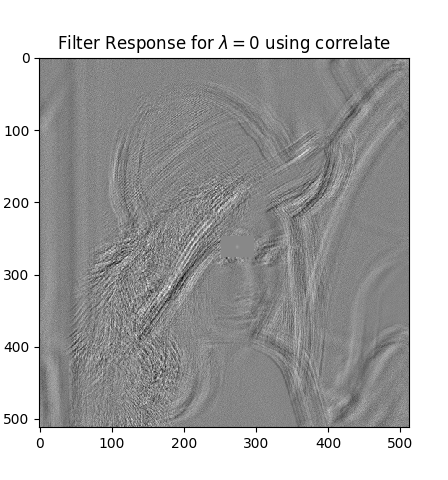
\includegraphics[width=0.35\textwidth]{corr-filters/g0_corr}} &
{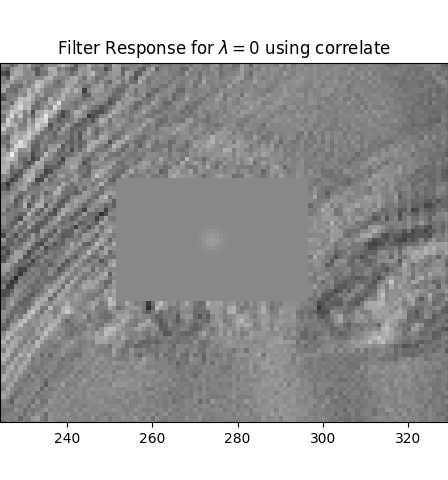
\includegraphics[width=0.35\textwidth]{corr-filters/g0_corr_zoom}}
\end{tabular}
\caption{Filter Response on Lena Image for $\lambda=0$, using Correlation}
\end{figure}

\begin{figure}[!ht]
\centering
\begin{tabular}{cc}
{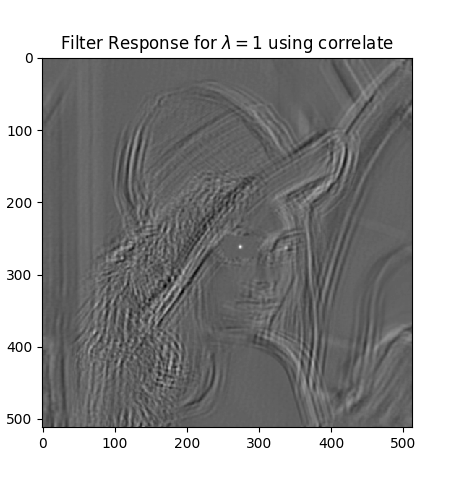
\includegraphics[width=0.35\textwidth]{corr-filters/g1_corr}} &
{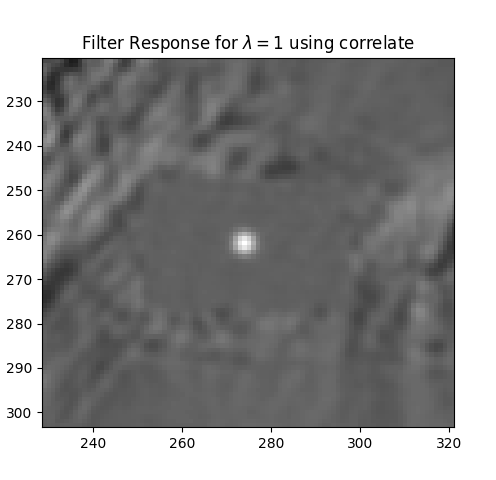
\includegraphics[width=0.38\textwidth]{corr-filters/g1_corr_zoom}}
\end{tabular}
\caption{Filter Response on Lena Image for $\lambda=1$, using Correlation}
\end{figure}

\begin{figure}[!ht]
\centering
{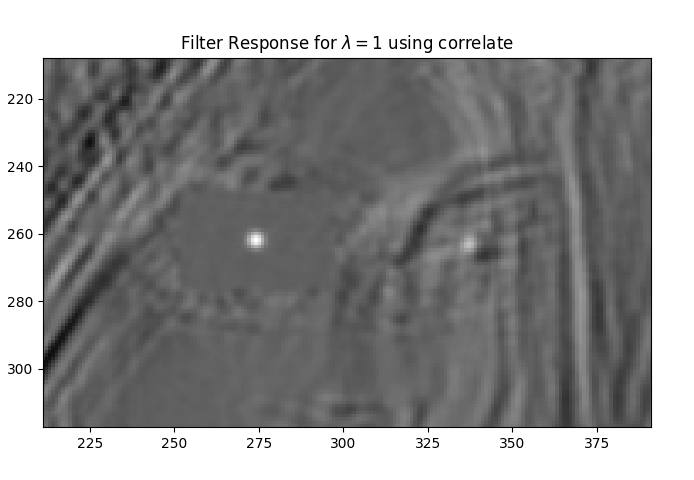
\includegraphics[width=0.7\textwidth]{corr-filters/g1_eyes}}
\caption{Filter Response on Lena Image for $\lambda=1$, showing responses on both the eyes}
\end{figure}

\newpage
The filter with $\lambda=1$ performs better because we are performing L2 regularization. In other words we can consider the second term as the radius of our trust region and thus would perform better by decreasing the overlap with the trust region. The regularization term helps us in creating an unique filter from the set of sub-images and thus we have a sharper response at the eye. 

The filter with $\lambda=0$ increases the area of the overlap with the trust region and disables the L2 regularization and hence it gives a blurry response around the eye, which means that the filter correlates with multiple sub-images with neither of them having a strong peak or a response.

\clearpage
\subsection{Filter Responses using Convolution}
Convolution is a mathematical sliding and window operation that generates some output based on the filter, which is flipped. Correlation is another sliding window dot product operation that measures the similarity between two images. This is the reason why we get the following responses with convolution.

Since in, convolution the only difference is that the filter is flipped, we can do this using Numpy indexing as follows.

\begin{center}
    \texttt{convolve(image, filter[::-1, ::-1])}
\end{center}

\begin{figure}[!ht]
\centering
\begin{tabular}{ccc}
{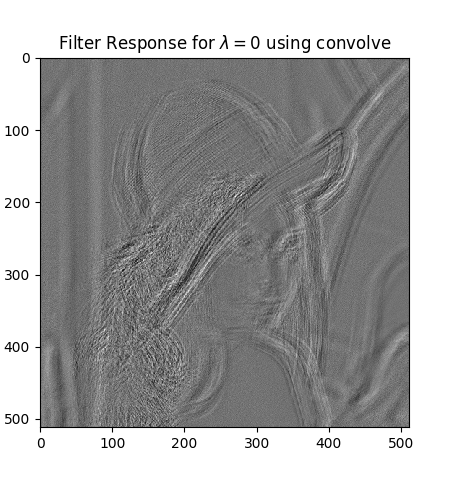
\includegraphics[width=0.3\textwidth]{corr-filters/g0_conv_non}} &
{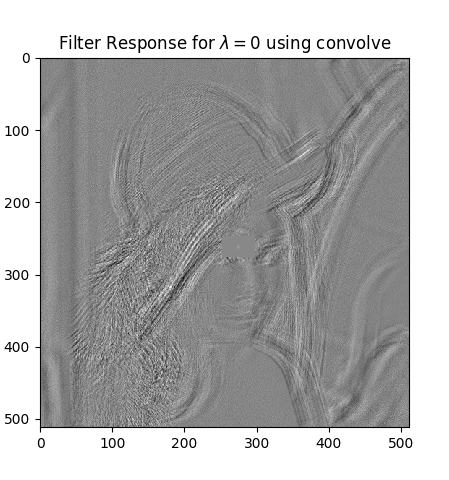
\includegraphics[width=0.3\textwidth]{corr-filters/g0_conv}} &
{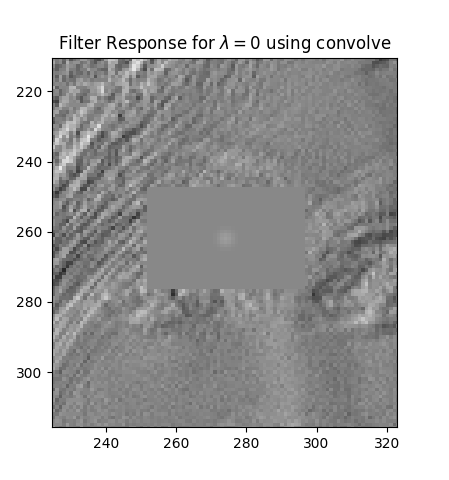
\includegraphics[width=0.3\textwidth]{corr-filters/g0_conv_zoom}}
\end{tabular}
\caption{Filter Response on Lena Image for $\lambda=0$, using Convolution and Flipped Filter Convolution}
\end{figure}

\begin{figure}[!ht]
\centering
\begin{tabular}{ccc}
{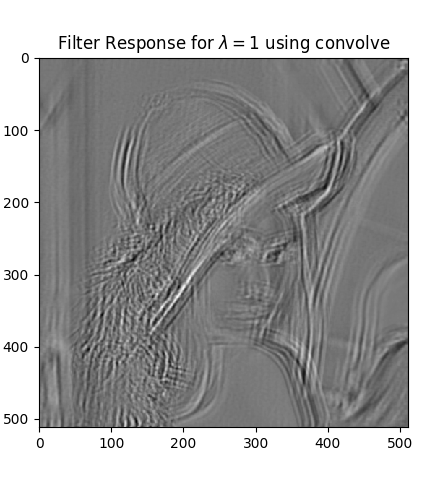
\includegraphics[width=0.3\textwidth]{corr-filters/g1_conv_non}} &
{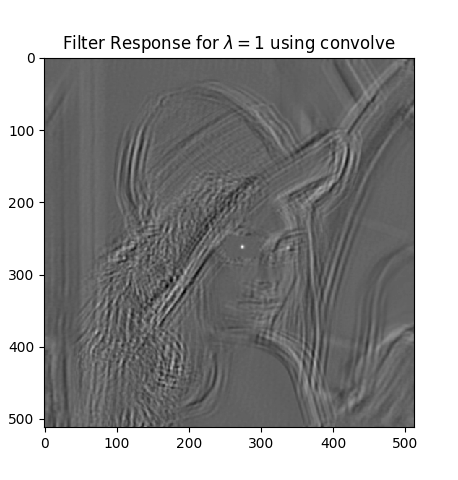
\includegraphics[width=0.3\textwidth]{corr-filters/g1_conv}} &
{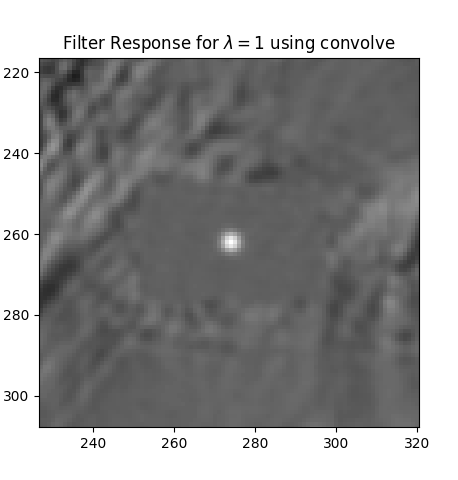
\includegraphics[width=0.3\textwidth]{corr-filters/g1_conv_zoom}}
\end{tabular}
\caption{Filter Response on Lena Image for $\lambda=1$, using Convolution and Flipped Filter Convolution}
\end{figure}

\end{document} 